\section{Voice Recording}
\subsection{Purpose}
This appendix describes the recording and subsequent manipulation of the sound used in the demonstration of the results of the project. The recording is in English. The speaker is a man with English as his secondary language. 

\subsection{AAU number list}
\begin{table}[H]
	\centering
	\ra{1.3}
	\begin{tabular}{ c c c } \toprule
		{Item}	& {Description} 						& {AAU-no}. \\ \bottomrule 
		1	& Røde NT2000 	& aau14440-00	\\
		2	& Sound card RME Fireface 802	& 86838 		\\
		3	& Computer running Matlab 2016a	 & 	NAN	\\
		\bottomrule
	\end{tabular}
	\caption{Table over equipment used for recording speech.}
	\label{tab:VoiceRec}
\end{table}

\subsection{Diagram}
\begin{figure}[H]
	\centering
	\tikzsetnextfilename{VoiceRecording}	
	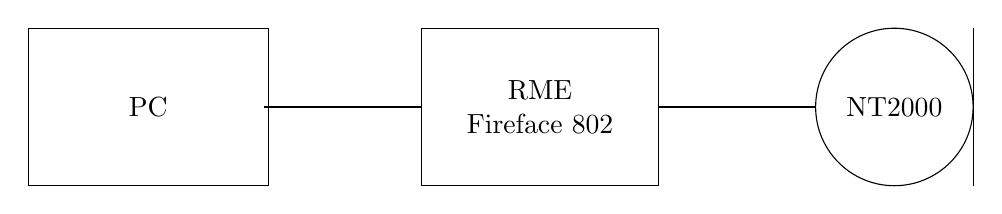
\begin{tikzpicture}
	\draw  (-2,1.5) rectangle (1.05,-0.5) node[pos=.5] {PC};
	\draw  (3,1.5) rectangle node[text width =2cm,text centered] {RME Fireface 802} (6,-0.5);
	\draw (1,0.5) -- (3,0.5);
	\draw  (9,0.5) ellipse (1 and 1)node[text width =1.75cm,text centered] {NT2000};
	\draw (10,1.5) -- (10,-0.5);
	\draw (8,0.5) -- (6,0.5);
	\end{tikzpicture}
	\caption{Voice recording set-up.}
	\label{fig:VoiceRecording}
\end{figure}

\subsection{Settings/Description}
The recording of speech is performed in an anechoic chamber, where a male speaker is situated 1 m from the microphone. The microphone is supplied with phantom power from the RME Fireface 802. \\ 

\subsection{Settings}
The parameters chosen for the recording, prediction and cancellation are:
\begin{itemize}
	\item $N=1200$
	\item $O=1100$
	\item $M=1200$
	\item $P=10$
	\item Delay equal to $P=10$
	\item $f_s =48000$ Hz
	\item $\mu=0.001$
\end{itemize}

\subsection{Performing the recording}
The manuscript is divided into sections, where different manipulations are made. Each section is stored in separate audio files for easier manipulation of the individual parts. The procedure of recording is:
\begin{itemize}
	\item The script "Record.m" is adjusted to record enough time for the section being recorded. 
	\item A countdown from 5 is made from the control room using the intercom. On "one" the following happens.
	\begin{itemize}
		\item The script "Record.m" is run from the control room.
		\item The speaker draws breath and prepares to read a section.
	\end{itemize}
	\item After the recorder has stopped the quality of the recording is checked. It should be clear, without noise and with correct pronunciation.
	\item The recording is repeated for all sections in the manuscript.  
\end{itemize}

\subsubsection{Record.m}
\begin{lstlisting}[language=MATLAB,caption=Record.m.]
fs=48000;
h=audiorecorder(fs,16,1);

record(h);
pause(10);
stop(h);
myrec=getaudiodata(h);

audiowrite('storefile.wav',myrec,fs);
\end{lstlisting}

\subsubsection{The manuscript}


\textbf{Normal voice}\\
\textit{This experience is best if you use a pair of headphones. 
This recording will demonstrate the performance of an Active Noise Control system, in a headphone using Filtered-$x$ Least Mean Squares combined with a Linear Prediction Algorithm. }


\textbf{Headphone filtered sound}\\
\textit{Now imagine that you have put on your headphones. I am speaking to you from the outside of the headphones.}

\textbf{FXLMS}\\
\textit{You have now activated the noise cancellation. This resembles the experience you would get from a noise canceling headphone, when a person is speaking from outside of the headphone. 
Here no prediction was used. Now the predictor is activated. }

\textbf{LP FXLMS}\\
\textit{This is the Filtered-x Least Means Squares combined with the Linear Prediction algorithm. This should be almost inaudible to you. }

\textbf{Normal voice 2}\\
\textit{In case you did not hear, you have just listened to the Filtered-x Least Means Squares combined with the Linear Prediction algorithm. We will now listen to the predictor without noise cancelling.}

\textbf{The predicted sound}\\
\textit{You are now listening to the predictor predicting 200 $\mu$s ahead in time. You are listening to an estimate of what I am going to say.}  

\textbf{Summary}\\
\textit{We hope you enjoyed the demonstration. Thank you for listening.}

%
\subsection{Data extraction}
The files are stored automatically by "Record.m". The file should be renamed to fit what's recorded. 
The sections in the manuscript are filtered in the following way and stored:
\begin{table}[H]
	\centering
	\ra{1.3}
	\begin{tabular}{ c c } \toprule
		{Section}				& {Manipulation} \\ \bottomrule 
		Normal Voice			& No manipulation  	\\
		Headphone filtered sound& Filtered with Headphone transfer function \\
		FXLMS					& Filtered with FXLMS	\\
		LP FXLMS 				& Filtered with LP FXLMS	\\
		Normal Voice 2			& No manipulation \\
		The predicted signal 	& The output of the predictor	\\
		Summary 				& No manipulation	\\
		\bottomrule
	\end{tabular}
	\caption{Manipulation of the different parts of the recording.}
	\label{tab:VoiceRecSections}
\end{table}



\subsection{Conclusion}
A recording has been made and the complete manipulated recording is available here: \\
\url{https://www.youtube.com/watch?v=nI_hGrxFV1A} 











